\documentclass[journal=acsodf,manuscript=article]{achemso}
\usepackage[version=4]{mhchem}
\usepackage{amsmath,amssymb}
\usepackage{graphicx}
\usepackage{booktabs}
\usepackage{siunitx}

% auto-generated in-text numbers; do not edit by hand
\newcommand{\splitRandomRow}{0.88}
\newcommand{\splitLigand}{0.20}
\newcommand{\splitSource}{-0.03}
\newcommand{\splitFamily}{-0.24}
\newcommand{\splitProspective}{0.70}
\newcommand{\nLigands}{93}
\newcommand{\nSources}{45}
\newcommand{\nFamilies}{20}
\newcommand{\recallGreedyRow}{1.00}
\newcommand{\recallGreedyLig}{0.82}
\newcommand{\recallRandomRow}{0.45}
\newcommand{\recallRandomLig}{0.95}
\newcommand{\bestRankModel}{gradient boosting}
\newcommand{\bestRankRho}{0.28}
\newcommand{\covRaw}{0.72}
\newcommand{\covConformal}{0.90}
\newcommand{\covMondrian}{0.87}
\newcommand{\covProspective}{0.88}
\newcommand{\rankCorr}{0.85}
\newcommand{\mceRaw}{0.103}
\newcommand{\mceConformal}{0.013}
\newcommand{\mceFold}{8}
\newcommand{\batchExploitRtwo}{0.29}
\newcommand{\batchExploitRecall}{1.00}
\newcommand{\batchExploreRtwo}{0.30}
\newcommand{\batchExploreRecall}{0.83}
\newcommand{\batchEIrecall}{0.98}
\newcommand{\batchEIRtwo}{0.13}
\newcommand{\selCorr}{0.63}
\newcommand{\selOverlap}{4}
\newcommand{\selNpareto}{4}
\newcommand{\selNlig}{63}
\newcommand{\selMax}{6.1}


\author{Krishna Harish}
\affiliation{Lawrence E. Elkins High School, Missouri City, Texas, USA}
\email{krishnaharish2009@gmail.com}

\title{Objective-Dependent Active Learning and Calibrated Uncertainty for
Sample-Efficient Discovery of Rare-Earth Extractants: A Benchmark on 1{,}202
Experimental Distribution Coefficients with Prospective Validation}

\abbreviations{AL,UQ,RF,DNN,logD}
\keywords{active learning, uncertainty quantification, conformal prediction,
solvent extraction, rare-earth separation, benchmark}

\begin{document}

\begin{abstract}
Measuring distribution coefficients ($\log D$) for rare-earth solvent extraction is
slow and expensive, making sample-efficient machine learning attractive, but the
practical questions of \emph{which} acquisition strategy to use, whether the
attendant uncertainty estimates can be trusted, and how well a model actually
generalises to new chemistry are rarely answered together on real data. We
benchmark active learning (AL) on 1{,}202 experimental $\log D$ measurements for
lanthanide extraction (\nLigands{} ligands, 14 lanthanides, \nSources{} literature
sources), with prospective validation on four independently synthesised ligands.
Five findings emerge, each on real data with multi-seed statistics. (i)~A plain
random forest reaches $R^2=0.94$/RMSE$=0.33$ on the published row-level validation
split, outperforming the previously reported deep network ($R^2=0.85$); however,
under leakage-controlled splits that forbid a ligand, source, or structural family
from appearing in both train and test, the estimate collapses (grouped-CV
$R^2=\splitLigand{}$ to $\splitSource{}$), so the in-distribution number is strongly
optimistic and realistic deployability is far lower. (ii)~The optimal AL acquisition
is \emph{objective-dependent}: exploitation recovers all top row-level extractants
(top-10 recall $=1.0$) but yields a biased, poorly predictive model, whereas
exploration/random gives the best predictive model but finds few of the best; no
strategy dominates both, and this survives a chemically realistic ligand-batch
acquisition unit and reproduces on an independent 4{,}200-compound $\log D$
benchmark. (iii)~The discovery ranking of strategies \emph{inverts} with the
definition of a ``top'' system: exploitation dominates for condition-specific rows,
but broad sampling already recovers most top ligands. (iv)~For \emph{prediction}, AL
provides no advantage over random selection. (v)~Conformal calibration is essential
for trustworthy uncertainty (an eight-fold in-distribution error reduction) but does
not improve AL acquisition, which depends only on the uncertainty ranking; under
distribution shift, global conformal leaves subgroup imbalance that group-conditional
(Mondrian) calibration reduces, at the cost of reordering the ranking. We compare
five model/uncertainty estimators, add early-recognition discovery metrics, and
distil the results into a practical decision guide, releasing all code and data.
\end{abstract}

\section{Introduction}
Separating rare-earth and $f$-elements by solvent extraction underpins critical-metal
supply and nuclear-fuel-cycle chemistry, and the key performance descriptor, the
distribution coefficient $\log D$, is measured one ligand/metal/condition at a time
by liquid--liquid assay.\cite{Panak_2013} Each measurement is laborious, so a model
that reaches useful accuracy, or surfaces the best extractants, from \emph{few}
measurements has direct practical value. Machine learning for $\log D$ and
distribution-coefficient prediction in rare-earth extraction has advanced
quickly,\cite{Liu_2022,Udawattha_2025,Chaube_2020,Edaugal_2025} and active learning
(AL)\cite{Settles_2009,Reker_2020} promises to choose the most informative
experiments next; pool-based AL with surrogate models has accelerated molecular
discovery and high-throughput screening,\cite{Graff_2021,Rohr_2020,Bayley_2024} and
batch acquisition is now standard when several experiments are run per
round.\cite{Bailey_2023}

Three practitioner-facing questions are nonetheless usually left unanswered on real
extractant data. First, \emph{which} acquisition strategy to use when the goal may be
accurate prediction \emph{or} discovery of top performers: the exploration
--exploitation trade-off is well studied in Bayesian
optimisation,\cite{DeAth_2021,Jones_1998,Shahriari_2016} and sequential-learning
benchmarks show the best scheme is goal-dependent and can even underperform
random,\cite{Rohr_2020} but this is rarely quantified for $f$-element separation.
Second, \emph{whether} the uncertainty estimates AL relies on are calibrated enough
to trust: conformal prediction gives distribution-free
guarantees\cite{Vovk_2005,Lei_2018,Angelopoulos_2023} and is increasingly used in
cheminformatics,\cite{Norinder_2014,Arvidsson_McShane_2024,Sun_2017} yet valid
average coverage can still hide failures in the high-$\log D$ region that matters most
for discovery. Third, \emph{how well} a model generalises beyond its training
chemotypes: random cross-validation is known to overstate prospective
performance,\cite{Sheridan_2013} and scaffold or cluster splits expose generalization
gaps that random splits hide.\cite{Wu_2018,Guo_2024,Guo_2025} We address all three on
a real benchmark of 1{,}202 experimental $\log D$ values with prospective validation,
and report findings that are useful precisely because several run counter to the
common framing of AL as a uniformly beneficial drop-in.

\section{Data and Methods}
\textbf{Dataset and recovered group structure.} We use the 1{,}202 experimental
lanthanide-extraction $\log D$ measurements compiled by Liu et
al.\cite{Liu_2022} (1{,}085 training $+$ 117 validation), with their feature
representation: Morgan/ECFP bits and RDKit physicochemical descriptors for the
ligand, experimental conditions (ligand and acid concentration, diluent
identity/ratio, temperature), and lanthanide-identity descriptors (2{,}291 features
per row). The released matrix contains no SMILES, but the group structure needed for
rigorous evaluation is recoverable from it: identical ECFP bit-vectors identify the
\nLigands{} unique ligands, the metal-descriptor block identifies the 14 lanthanides,
and the integer citation index identifies the \nSources{} publication sources (median
14 measurements and 9 distinct lanthanides per ligand). Their four subsequently
synthesised ligands (56 ligand$\times$metal measurements) serve as a strictly
prospective external test.

\textbf{Leakage-controlled splits.} Because random row-level cross-validation can
place measurements of the same ligand or source in both train and test, we evaluate
generalisation under four regimes with identical models: plain 5-fold over rows, and
group-disjoint 5-fold (repeated with reshuffled group assignments) that forbid a
shared \emph{ligand}, \emph{source}, or structural \emph{family}. Exact Bemis--Murcko
scaffolds require SMILES that are not distributed, so we use ECFP-Tanimoto
agglomerative clustering (\nFamilies{} families at similarity $\ge 0.35$) as an
explicit scaffold-split proxy.

\textbf{Surrogate, models, and uncertainty.} The base model is a random-forest
regressor\cite{Breiman_2001} (scikit-learn\cite{Pedregosa_2011}); epistemic
uncertainty is the standard deviation across trees, an ensemble estimator in the
spirit of deep ensembles.\cite{Lakshminarayanan_2017,Scalia_2020,Hirschfeld_2020} To
probe whether the conclusions depend on this choice we additionally benchmark a
quantile regression forest, a Gaussian process (on PCA-reduced features), gradient
boosting, and a Monte-Carlo-dropout Bayesian neural
network,\cite{Gal_2016,Soleimany_2021,Busk_2022} scored on predictive accuracy,
calibration, and uncertainty-ranking quality. We apply split-conformal
calibration\cite{Vovk_2005,Lei_2018,Angelopoulos_2023} (nonconformity
$|y-\hat{y}|/\hat\sigma$ on a held-out calibration split), and, for subgroup
coverage, group-conditional (Mondrian) conformal prediction.\cite{Sun_2017}

\textbf{Active-learning protocol.} From a small random seed set we iteratively acquire
batches and retrain. We use two acquisition units: the original row unit
(fixed $80/20$ pool/test partition) and a chemically realistic \emph{ligand-batch}
unit, in which selecting a ligand reveals all of its measurements at once and the
test set is a disjoint set of held-out ligands. Acquisition strategies: \emph{random};
\emph{greedy} (exploit, maximise predicted $\log D$); \emph{uncertainty} (explore,
maximise $\hat\sigma$); \emph{UCB} ($\hat\mu+1.5\hat\sigma$); \emph{expected
improvement} (EI)\cite{Jones_1998,Shahriari_2016}; and a \emph{hybrid} portfolio
(half exploit, half explore). We track, versus number of measurements, the held-out
predictive $R^2$ and discovery metrics: top-10 recall under three definitions of a
``top system'' (condition-specific row, ligand--metal pair, unique ligand), the
enrichment factor,\cite{Truchon_2007,Ash_2022} simple regret, and hit-rate above a
practical threshold ($\log D\ge 1$, i.e.\ $D\ge 10$). All curves are averaged over six
random seeds.

\section{Results and Discussion}
\textbf{A strong but optimistic simple baseline.} A random forest on the published
features attains $R^2=0.942$, RMSE$=0.328$ on the published validation split,
exceeding the reported deep network ($R^2=0.85$, RMSE$=0.53$).\cite{Liu_2022} For this
tabular, condition-rich representation, ensemble trees are a stronger and far cheaper
baseline. This comparison is on the same row-level split as the original, and is
therefore an apples-to-apples model comparison, not an estimate of deployability.

\textbf{Realistic generalisation under leakage-controlled splits
(Figure~\ref{fig:splits}, Table~\ref{tab:splits}).} The row-level number is
strongly optimistic. Holding out entire ligands, sources, or structural families
collapses the estimate from $R^2=\splitRandomRow{}$ (random rows) to
$R^2=\splitLigand{}$ (ligand-disjoint), $\splitSource{}$ (source-disjoint), and
$\splitFamily{}$ (family-disjoint), i.e.\ to at or below the performance of predicting
the mean. The prospective test on four genuinely new ligands gives
$R^2=\splitProspective{}$, intermediate between the two extremes because those ligands
are close analogues of training chemotypes. The practical implication is that
in-distribution $R^2$ on this benchmark should not be read as deployability; realistic
generalisation to new ligand chemistry is markedly lower, consistent with the
random-split optimism documented across molecular ML.\cite{Sheridan_2013,Guo_2024}

\begin{figure}[htbp]\centering
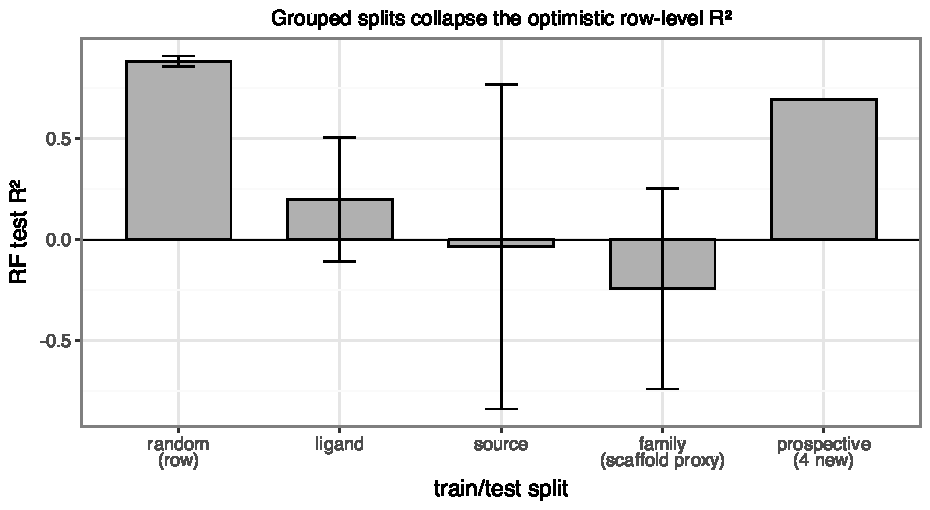
\includegraphics[width=0.72\linewidth]{../figures/splits.pdf}
\caption{Random-forest test $R^2$ under increasingly stringent, leakage-controlled
splits. Random row-level CV is strongly optimistic; grouped splits that forbid a
shared ligand, source, or structural family collapse the estimate toward the mean.
Error bars are $\pm1$ s.d.\ over repeated grouped folds.}
\label{fig:splits}
\end{figure}

\begin{table}[htbp]
\centering
\caption{Random-forest generalisation under increasingly stringent, leakage-controlled splits. Random row-level cross-validation is strongly optimistic; grouped splits that forbid a ligand, source, or structural family from appearing in both train and test collapse the estimate toward the mean. Mean$\pm$s.d.\ over 4 repeats of 5-fold grouped CV.}
\label{tab:splits}
\begin{tabular}{lccc}
\toprule
Split & $R^2$ & RMSE & MAE \\
\midrule
Random (row-level) & 0.88$\pm$0.03 & 0.46 & 0.28 \\
Ligand-disjoint & 0.20$\pm$0.31 & 1.14 & 0.87 \\
Source-disjoint & -0.03$\pm$0.80 & 1.22 & 0.98 \\
Ligand-family (scaffold proxy) & -0.24$\pm$0.50 & 1.31 & 1.04 \\
\midrule
Prospective (4 new ligands) & 0.70 & 0.63 & 0.49 \\
\bottomrule
\end{tabular}
\end{table}


\textbf{The optimal acquisition is objective-dependent (Figure~\ref{fig:al}).} No
single strategy is best. Exploitation (greedy, UCB) recovers \emph{all} top row-level
extractants (top-10 recall $=1.00$) but biases the training set toward high-$\log D$
systems, giving a poor global model ($R^2=0.63$--$0.70$). Exploration and random give
the best predictive models ($R^2=0.85$--$0.87$) but poor row-level design recall
($0.38$--$0.50$). EI and the hybrid portfolio sit on the Pareto front but dominate
neither extreme. Practitioners must therefore choose the acquisition by the goal:
exploit to \emph{find} extractants, explore to \emph{model} them, EI/hybrid to
balance. This matches sequential-learning benchmarks in which the best scheme is
goal-dependent and mismatched schemes underperform random.\cite{Rohr_2020,DeAth_2021}

\begin{figure}[htbp]\centering
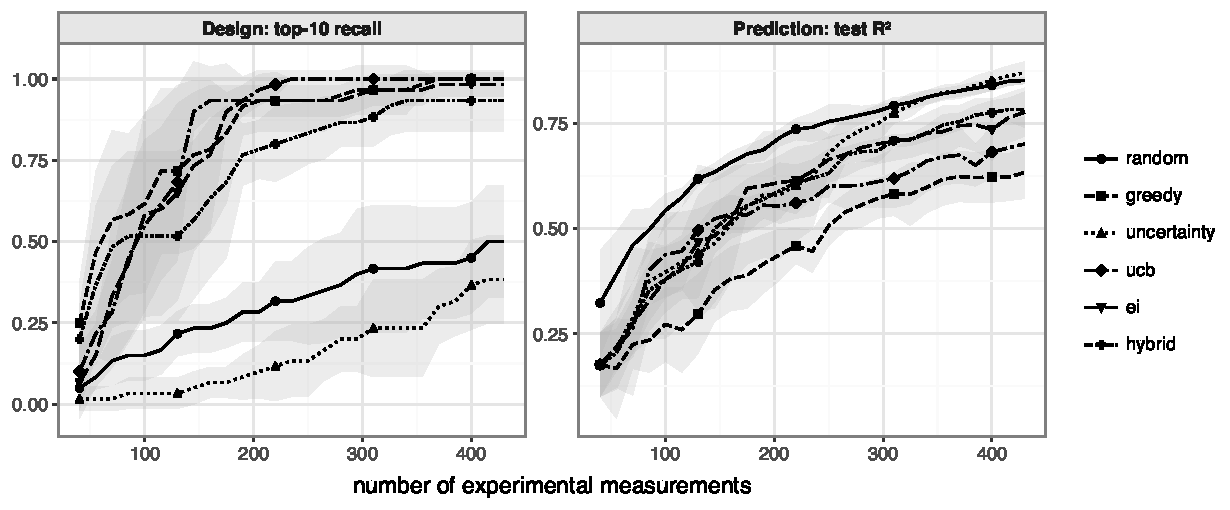
\includegraphics[width=0.92\linewidth]{../figures/real_al.pdf}
\caption{Active learning on 1{,}202 real $\log D$ measurements (row unit). Left:
predictive $R^2$ vs.\ number of measurements (exploration/random best). Right: top-10
recall (exploitation best). No strategy wins both; EI and the hybrid portfolio trace
the Pareto front. Bands are $\pm1$ s.d.\ over six seeds.}
\label{fig:al}
\end{figure}

\textbf{The dichotomy survives a realistic ligand-batch unit
(Figure~\ref{fig:batch}).} In the laboratory one selects a \emph{ligand} and then
measures it against many lanthanides and conditions, so we repeat the benchmark with a
ligand-batch acquisition unit and a ligand-disjoint test set. The design-side
dichotomy is clear: exploitation reaches the highest top-10 ligand recall
($\batchExploitRecall{}$) while random/exploration lags on recall
($\batchExploreRecall{}$). On the prediction side, all predictive $R^2$ are low under
this deliberately hard ligand-disjoint test (consistent with the split analysis
above), with random giving the best model ($R^2=\batchExploreRtwo{}$) but by a small
margin over exploitation ($\batchExploitRtwo{}$). The objective-dependent ordering is
therefore preserved under the operational decision unit, not an artefact of scoring
isolated rows, though the prediction-side gap narrows once the test set forbids
train--test ligand overlap.

\begin{figure}[htbp]\centering
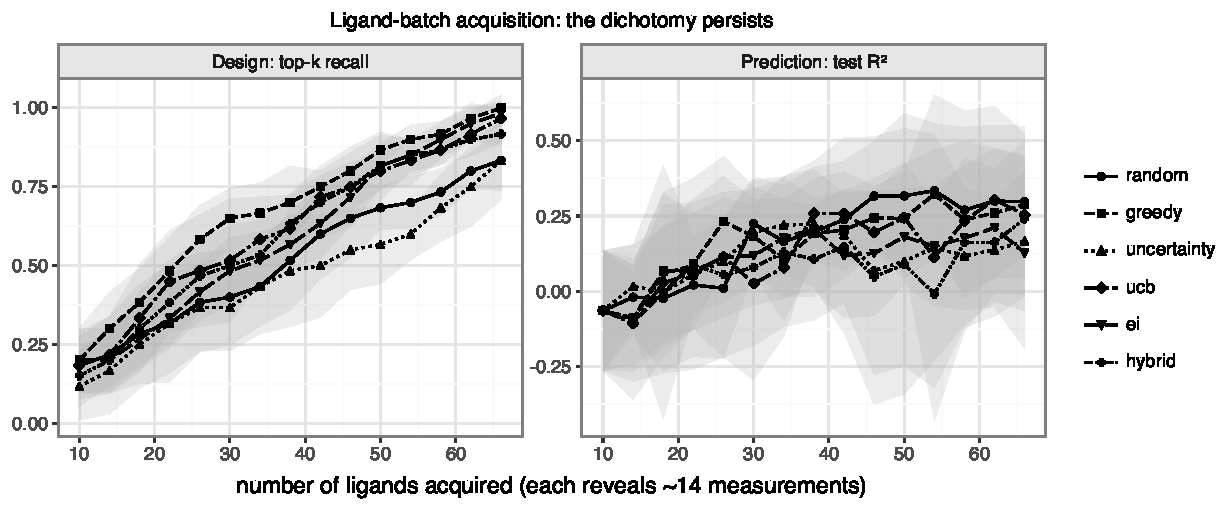
\includegraphics[width=0.92\linewidth]{../figures/ligand_batch.pdf}
\caption{Ligand-batch acquisition (each acquired ligand reveals $\sim$14 measurements),
with a ligand-disjoint test set. Left: predictive $R^2$; right: top-10 ligand recall.
The objective-dependent dichotomy persists under the realistic decision unit. Bands
are $\pm1$ s.d.\ over six seeds.}
\label{fig:batch}
\end{figure}

\textbf{What counts as a ``top'' system changes the ranking
(Figure~\ref{fig:recalldef}, Table~\ref{tab:recall}).} Discovery value depends on
whether a top system is a condition-specific row, a ligand--metal pair, or a unique
ligand, and the strategy ranking \emph{inverts} across these definitions. Exploitation
dominates at the row level (greedy row-recall $\recallGreedyRow{}$ vs random
$\recallRandomRow{}$), because it targets the exact high-$\log D$ conditions. But at the
ligand level the ordering flips: broad sampling already recovers most top ligands
(random ligand-recall $\recallRandomLig{}$ vs greedy $\recallGreedyLig{}$), because
each ligand appears under many conditions and is therefore easy to hit without
targeting. Reporting a single ``top-10 recall'' without stating the unit can thus
reverse the practical conclusion; we report all three.

\begin{figure}[htbp]\centering
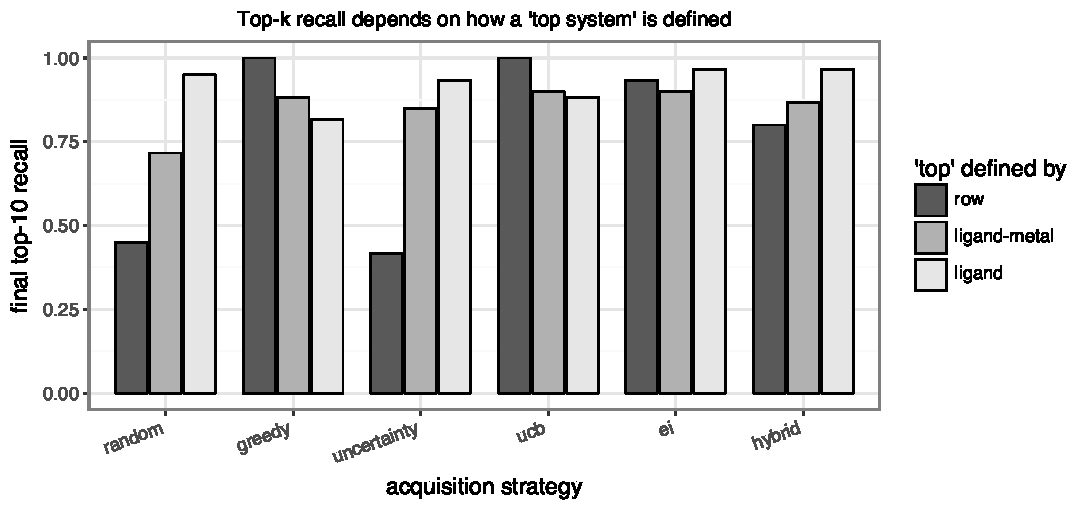
\includegraphics[width=0.85\linewidth]{../figures/recall_defs.pdf}
\caption{Final top-10 recall under three definitions of a ``top'' system. Exploitation
is best for condition-specific rows; broad/random sampling is competitive or better
for unique ligands. The discovery conclusion depends on the definition.}
\label{fig:recalldef}
\end{figure}

\begin{table}[htbp]
\centering
\caption{Discovery performance at the final budget under three definitions of a `top-10 system' (condition-specific row, ligand--metal pair, unique ligand), plus simple regret (log units) and hit-rate above a practical threshold ($\log D\ge 1$, i.e.\ $D\ge 10$). The ranking of strategies inverts with the definition: exploitation dominates for rows, but broad sampling already recovers most top ligands. Means over six seeds.}
\label{tab:recall}
\begin{tabular}{lccccc}
\toprule
Strategy & recall & recall & recall & regret & hit-rate \\
 & (row) & (lig--metal) & (ligand) & (log) & ($\log D\!\ge\!1$) \\
\midrule
random & 0.45 & 0.72 & 0.95 & 0.15 & 0.26 \\
greedy & 1.00 & 0.88 & 0.82 & 0.00 & 0.60 \\
uncertainty & 0.42 & 0.85 & 0.93 & 0.12 & 0.26 \\
ucb & 1.00 & 0.90 & 0.88 & 0.00 & 0.59 \\
ei & 0.93 & 0.90 & 0.97 & 0.02 & 0.47 \\
hybrid & 0.80 & 0.87 & 0.97 & 0.01 & 0.52 \\
\bottomrule
\end{tabular}
\end{table}


\textbf{The dichotomy is general (Figure~\ref{fig:lipo}).} On an independent dataset,
the 4{,}200 octanol--water $\log D$ values from MoleculeNet's Lipophilicity
set\cite{Wu_2018} with a different feature representation, the same anti-correlated
pattern emerges: exploration and random give the best predictive models
($R^2\approx0.50$) but the lowest design recall ($0.20$--$0.27$), whereas exploitation
gives the best recall ($0.53$--$0.57$) but the worst predictive models
($R^2=0.21$--$0.28$). The objective-dependence of the optimal acquisition is therefore
a general property of pool-based AL, not an artefact of one dataset or feature set.

\begin{figure}[htbp]\centering
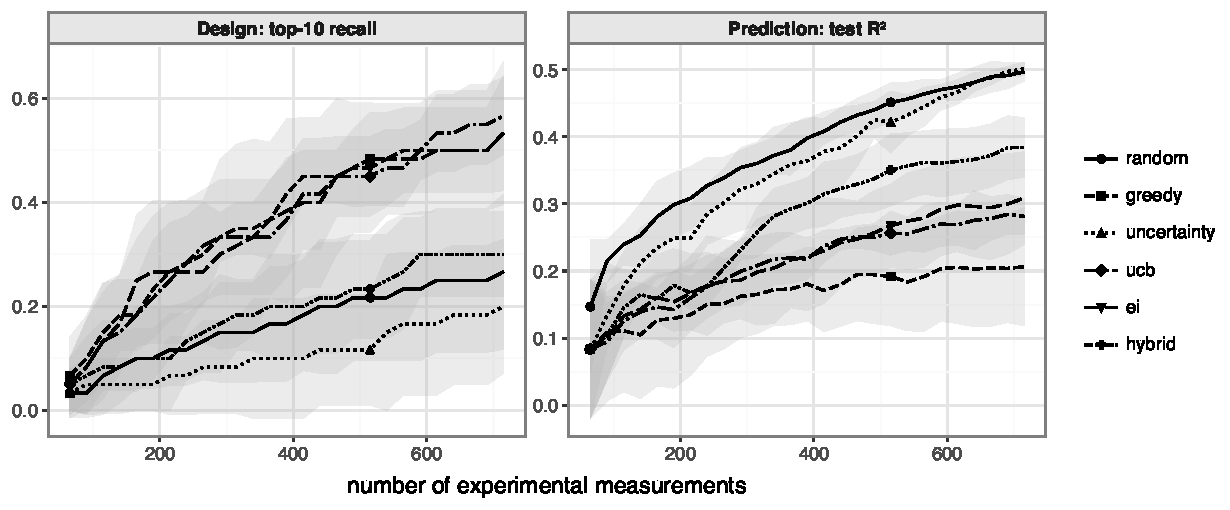
\includegraphics[width=0.92\linewidth]{../figures/lipo_al.pdf}
\caption{Generality. The identical prediction--design dichotomy on an independent
benchmark (4{,}200 octanol--water $\log D$ values, Morgan-fingerprint features).}
\label{fig:lipo}
\end{figure}

\textbf{Active learning does not help prediction (a caution).} At every budget, random
selection matches or beats uncertainty sampling for predictive $R^2$ (e.g.\ $0.54$ vs
$0.40$ at 100 measurements; both reach $R^2=0.85$ at $\approx400$). For building a
predictive $\log D$ model, the experimental effort of AL is not repaid here, echoing
UQ comparisons in which no acquisition uniformly helps.\cite{Hirschfeld_2020}

\textbf{Calibration matters for trust, not acquisition
(Figure~\ref{fig:calsub}, Table~\ref{tab:calib}).} On the row-level split, raw
ensemble uncertainty is badly miscalibrated (mean calibration error $\mceRaw{}$; the
nominal-$80\%$ interval covers $90\%$), and split-conformal calibration reduces the
error \mceFold{}-fold to $\mceConformal{}$. Yet calibrating the uncertainty leaves AL
performance unchanged, because acquisition depends only on the \emph{ranking} of
uncertainty, which a single global (monotone) conformal factor preserves. Under a
realistic ligand-disjoint split the picture is richer: raw intervals now
\emph{under}-cover ($\covRaw{}$ at nominal $0.80$), a single global conformal factor
restores average coverage ($\covConformal{}$) but leaves the high-$\log D$ region
unevenly covered, and group-conditional (Mondrian) conformal
($\covMondrian{}$)\cite{Sun_2017} evens the subgroups. Crucially, Mondrian
\emph{reorders} the uncertainty ranking (Spearman $\rho=\rankCorr{}$ vs the global
factor), so locally adaptive calibration \emph{can} change AL acquisition even though a
global factor cannot. Coverage on the prospective ligands is $\covProspective{}$.
Calibration is thus essential when the uncertainty is reported or acted
upon\cite{Janet_2019,Yang_2023}, and, for acquisition, only non-monotone calibration
matters, a distinction easy to conflate.

\begin{figure}[htbp]\centering
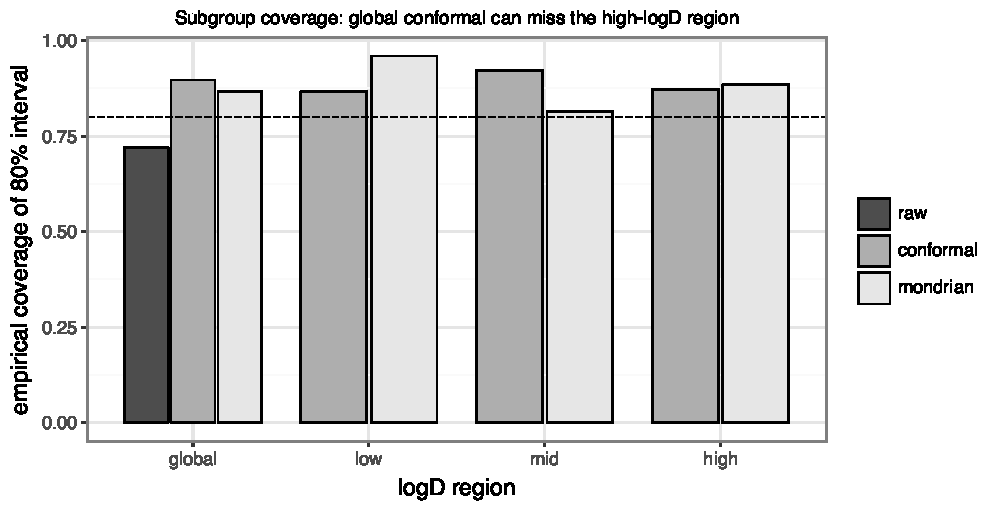
\includegraphics[width=0.8\linewidth]{../figures/calibration_subgroups.pdf}
\caption{Subgroup coverage of nominal-$80\%$ intervals under a ligand-disjoint split.
Raw intervals under-cover; a single global conformal factor restores average coverage
but the high-$\log D$ region remains uneven; group-conditional (Mondrian) conformal
balances the subgroups. Dashed line is the nominal target.}
\label{fig:calsub}
\end{figure}

\begin{table}[htbp]
\centering
\caption{Uncertainty calibration under a realistic ligand-disjoint split (nominal coverage 80\%). Raw ensemble intervals under-cover; a single global split-conformal factor restores average coverage but leaves subgroup imbalance, which group-conditional (Mondrian) conformal reduces. Mean over eight seeds. For reference, on the easier row-level split the raw mean calibration error is 0.103 and conformal reduces it to 0.013.}
\label{tab:calib}
\begin{tabular}{lcccc}
\toprule
Method & global & low $\log D$ & mid $\log D$ & high $\log D$ \\
\midrule
Raw & 0.72 & -- & -- & -- \\
Global conformal & 0.90 & 0.87 & 0.92 & 0.87 \\
Mondrian conformal & 0.87 & 0.96 & 0.82 & 0.88 \\
\bottomrule
\end{tabular}
\end{table}


\textbf{Broader model and uncertainty-estimator baselines (Table~\ref{tab:uq},
Figure~\ref{fig:uq}).} To test whether the conclusions depend on the random forest, we
compare five estimators on a ligand-disjoint split: random forest, quantile regression
forest, Gaussian process, gradient boosting, and an MC-dropout Bayesian neural
network. No estimator uniformly dominates, consistent with prior UQ
comparisons;\cite{Hirschfeld_2020,Scalia_2020} \bestRankModel{} gives the best
uncertainty-ranking quality (Spearman between predicted $\sigma$ and realised absolute
error, $\rho=\bestRankRho{}$). The dichotomy and the calibration-vs-acquisition
distinction are properties of pool-based AL, not of a single surrogate.

\begin{figure}[htbp]\centering
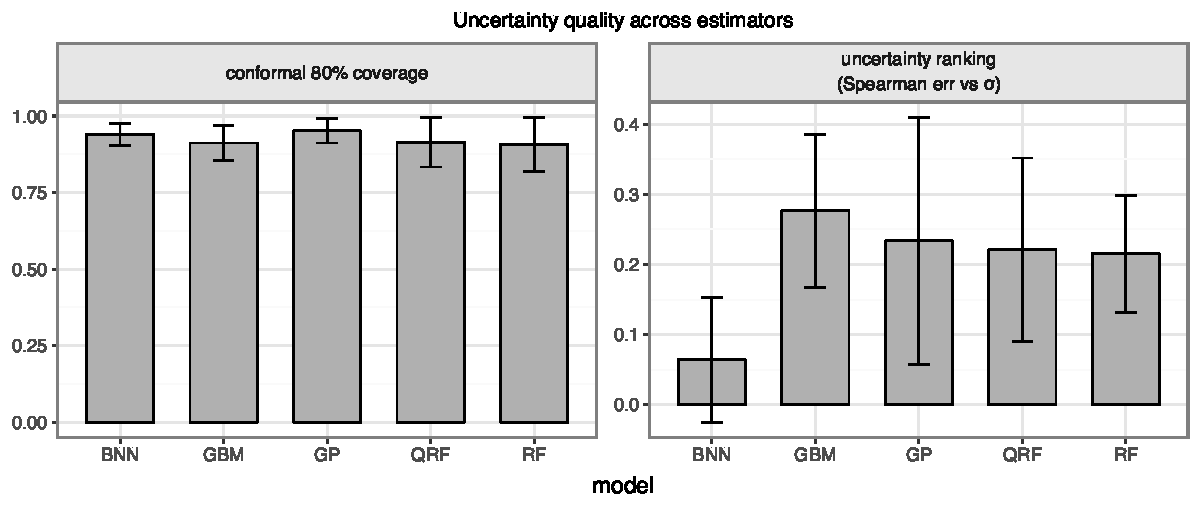
\includegraphics[width=0.9\linewidth]{../figures/uq_models.pdf}
\caption{Model/uncertainty-estimator comparison on a ligand-disjoint split: conformal
$80\%$ coverage and uncertainty-ranking quality (Spearman of predicted $\sigma$ vs
realised error). Error bars are $\pm1$ s.d.\ over four seeds.}
\label{fig:uq}
\end{figure}

\begin{table}[htbp]
\centering
\caption{Model and uncertainty-estimator comparison on a ligand-disjoint split (train/calibration/test $=55/20/25$ of ligands). Uncertainty-ranking quality is the Spearman correlation between predicted $\sigma$ and realised absolute error; higher is better. Coverage is the empirical coverage of split-conformal 80\% intervals. Mean over four seeds.}
\label{tab:uq}
\begin{tabular}{lcccc}
\toprule
Model & $R^2$ & conformal & rank quality & enrich. \\
 & & 80\% cov. & $\rho(|e|,\sigma)$ & factor \\
\midrule
Random forest & 0.15 & 0.91 & 0.22 & 7.5 \\
Quantile RF & 0.14 & 0.91 & 0.22 & 7.5 \\
Gaussian process & -0.03 & 0.95 & 0.23 & 3.7 \\
Gradient boosting & 0.22 & 0.91 & 0.28 & 7.5 \\
MC-dropout BNN & 0.12 & 0.94 & 0.06 & 6.6 \\
\bottomrule
\end{tabular}
\end{table}


\textbf{A high $\log D$ is not sufficient: selectivity
(Figure~\ref{fig:sel}).} In separations chemistry the objective is not a large
distribution coefficient per se but \emph{discrimination} between lanthanides. For each
of the \selNlig{} ligands measured against at least five lanthanides we compute a
separation factor as the spread of $\log D$ across metals (the log of the best/worst
distribution-coefficient ratio), which spans up to \selMax{} log units. Ranking
ligands by extraction strength (max $\log D$) is not the same as ranking by
selectivity: the two correlate only moderately (Spearman $\selCorr{}$), and only
\selOverlap{} of the top-10 strongest extractants are also among the top-10 most
selective. Optimising $\log D$ alone therefore misses most of the discriminating
ligands, and the design objective (and any AL acquisition built on it) should target
selectivity directly; the $\selNpareto{}$ Pareto-optimal ligands in the
strength--selectivity plane are the appropriate design targets. A full multi-objective
selectivity-aware acquisition is a natural extension of this benchmark.

\begin{figure}[htbp]\centering
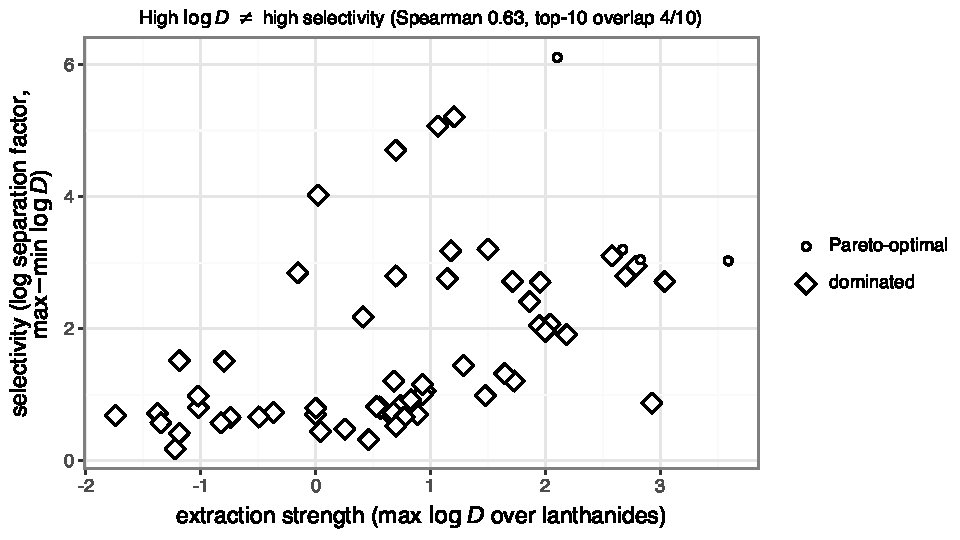
\includegraphics[width=0.7\linewidth]{../figures/selectivity.pdf}
\caption{Extraction strength (max $\log D$) versus selectivity (log separation factor,
max$-$min $\log D$ across lanthanides) for each ligand. The two are only moderately
correlated, so a high $\log D$ does not imply a selective extractant; diamonds mark the
Pareto-optimal ligands.}
\label{fig:sel}
\end{figure}

\textbf{Prospective validation.} Trained on all 1{,}202 measurements and applied to the
four independently synthesised ligands, the model attains $R^2=\splitProspective{}$,
RMSE$=0.639$, MAE$=0.502$ log units. Read together with the grouped-CV collapse above,
this places realistic generalisation between the optimistic row-level number and the
worst-case family-held-out number, and is, to our knowledge, among the few prospective
tests reported for extractant-property models.

\textbf{Practical guidance.} (1)~Start with an ensemble-tree baseline, but report a
leakage-controlled (ligand/source/scaffold) split, not row-level CV, as the
generalisation estimate. (2)~Pick the acquisition by objective: exploit for discovery,
explore/random for a predictive model, EI for balance. (3)~State the unit of a ``top''
system; the discovery ranking depends on it. (4)~Do not expect AL to reduce the
measurements needed for accurate prediction. (5)~Calibrate (e.g.\ conformally) whenever
the uncertainty is reported or acted upon, and use group-conditional calibration when
subgroup coverage matters; only non-monotone calibration changes acquisition.
(6)~When the goal is separation, optimise selectivity (the $\log D$ spread across
metals), not $\log D$ alone: the two rankings diverge.

\section{Limitations}
The objective-dependent dichotomy is shown on two independent datasets with different
feature sets, but broader chemistries remain to be tested. Because SMILES are not
distributed with the benchmark, our structural split uses ECFP-Tanimoto families as a
scaffold-split proxy rather than exact Bemis--Murcko scaffolds. AL here is pool-based
selection over measured candidates, not open-ended generative design, and prospective
validation covers four ligands. We characterise selectivity (the spread of $\log D$
across lanthanides) and show it diverges from raw $\log D$, but a full multi-objective,
selectivity-aware acquisition loop is left as an extension; the conclusions concern
$\log D$ regression and may differ for classification targets.

\section{Conclusion}
On real experimental extractant data with prospective validation, we show that a
simple ensemble beats a published deep network but that row-level $R^2$ is strongly
optimistic relative to leakage-controlled splits; that the best active-learning
acquisition depends on whether the goal is prediction or discovery, with no strategy
dominating both, and that this survives a realistic ligand-batch unit while the
discovery ranking itself depends on how a ``top'' system is defined; that active
learning offers no predictive-accuracy advantage over random selection; and that
uncertainty calibration is essential for trust but changes acquisition only when it is
non-monotone. These give practitioners an evidence-based decision guide and a
reproducible benchmark for sample-efficient extractant discovery.

\section*{Data and Software Availability}
All analysis code, recovered group labels, split definitions, and figure- and
number-generating scripts are released at
\url{https://github.com/krishnatheaverage/logd-active-learning-benchmark} and archived
on Zenodo, reproducing every value herein on a single laptop. The underlying
measurements are from ref.~\citenum{Liu_2022}.

\begin{acknowledgement}
Computations were run on a single Apple M4 laptop. The author conceived and directed
the study, curated the data, made the scientific and methodological decisions, and
verified all results; in accordance with ACS policy, the author discloses that a
generative AI assistant (Claude, Anthropic) was used under the author's direction for
code implementation, experiment execution and analysis, and manuscript drafting. The
author is accountable for the content.
\end{acknowledgement}

\clearpage
\bibliography{refs_b}

\end{document}
